\chapter{Material Parameter Identification}%
\label{chapter:four}
The finite viscoelastic material model decribed in \cref{sec:finite_viscoelasticity} is characterized by a set of material parameters. For the response of the implemented material model to be in close agreement with real materials, these parameters need to be identified. The task of identifying suitable parameters of the finite viscoelastic model such that it is able to resemble a dual cross-link self-healing hydrogel is dealt with in this chapter.

\section{Material Parameters}
The parameters of the viscoelastic material model comprise of parameters from the elastic and viscous (inelastic) parts. As we have considered a Ogden class of strain energy of the first order, the set of parameters required to fully describe the model with \(k\) relaxation mechanisms is given by
\begin{equation}
\bm{x}_p = \left[\mu,\,\alpha,\,\K,\,(\mum,\,\am,\,\km,\,\nd,\,\nv)^{k}\right]^{T} 
\label{eq:parameters}  
\end{equation}
where 
\(\bm{x}_p\) is the parameter vector and the total number of parameters is given by \(3+5k\). Thus, for a viscoelastic model with two relaxation mechanisms \((k=2)\), the material model is characterized by 13 parameters in total. Furthermore, the viscosity parameters \(\nd\) and \(\nv\) can be given by 
\begin{align}
    \nd &= \mu_{vis} \tau_{r} = \mum \am \tau_{r} \label{eq:nd_rtime}\\
    \nv &= \km \tau_{r} \label{eq:nv_rtime}
\end{align}
where \(\tau_{r}\) is the relaxation time~\cite{Kleuter2007Jul}. The set of parameters can thus be reduced to 
\begin{equation}
    {\hat{\bm{x}}_p} = {\left[\mu,\,\alpha,\,\K,\,(\mum,\,\am,\,\km,\,\tau_{r}){}^{k}\right]}^{T}   
    \label{eq:parameters_red}
\end{equation}
where the total number of parameters can now be given by \(3 + 4k\).
As it will be seen further, reducing the number of the material parameters in this way benefits to the parameter identification procedure. 

\section{Experimental Data}
In order to find a suitable set of parameters as described in \cref{eq:parameters_red} of the viscoelastic material model, experimental data is required. However, performing experiments and collecting test data is a very time consuming process. Here, experimental data from uniaxial tension tests for a dual cross-link self-healing hydrogel is taken from \citeauthor{Long2014Oct} \cite{Long2014Oct}. In total, data from five experiments that were carried out at constant stretch rates varying from \(0.1s^{-1}\) to \(0.003s^{-1}\) as shown in \cref{fig:uniaxial_experiments} were used. At every time step \(t\), the data contained a value for nominal stress \(\sigma_{\text{nom}}\) or \(\mathrm{P_{11}}{|}_{\text{exp}}\) and stretch \(\prstretche{}{}\) in the axial direction of the test.
\begin{figure}[htbp]
    \centering
    \includegraphics[width=0.85\textwidth]{ExperimentalData}
    \caption[Experimental data for a hydrogel]{Uniaxial tension experimental data of a hydrogel.}%
    \label{fig:uniaxial_experiments}
\end{figure}

\section{Non-Linear Least-Squares Optimization}
The goal of the parameter identification procedure is to find the set of paramaters for which the error between the experimental data and simulation is minimized. This then reduces to a non-linear least-squares optimization problem, in which a cost function is minimized over a set of variables (material parameters). Here, the cost function is given by 
\begin{equation}
    \text{Cost}({\hat{\bm{x}}_p}) = \sum_{j=1}^{E} \sum_{i=1}^{N} \big|\big|(\mathbf{P}{|}_{\text{exp}})^{j}_{i} - (\mathbf{P}{|}_{\text{sim}})^{j}_{i} \big|\big|
\end{equation}
where \(\mathbf{P}\) is the first Piola-Kirchoff stress tensor \cref{eq:def_firstpiolakirchoffstress} representing the nominal stress, \(E\) is the total number of experiments, \(N\) is the number of data points within an experiment, and \(||\bullet||\) is the Frobenius norm. In the case of uniaxial tension this reduces to 
\begin{equation}
    \text{Cost}({\hat{\bm{x}}_p}) = \sum_{j=1}^{E} \sum_{i=1}^{N} \,\big|\big|\,(\mathrm{P_{11}}{|}_{\text{exp}})^{j}_{i} - (\mathrm{P}_{11}{|}_{\text{sim}})^{j}_{i}\,\big|\big|
\end{equation}
The optimization problem can be then written as
\begin{equation}
   \underset{{\hat{\bm{x}}_p}}{\text{argmin }} \text{Cost}({\hat{\bm{x}}_p})
   \label{eq:constrained_optimization_cost}
\end{equation}
additionally, subject to constraints 
\begin{equation}
    \K> 0 \quad \text{ and } \quad (\km)^{k} > 0
    \label{eq:constraint_1}
\end{equation}
\begin{equation*}
    \mathrm{sgn}(\mu) = \text{sgn}(\alpha)  \quad \text{ and } \quad \mathrm{sgn}(\mum)^{k} = \text{sgn}(\am)^{k}
\end{equation*}
or 
\begin{equation}
\mu \alpha > 0 \quad \text{ and } \quad (\mum)^{k}(\am)^{k} > 0
\label{eq:constraint_2}
\end{equation}
since the bulk and shear modulus cannot have a negative value. In general, \cref{eq:constraint_1}  and \cref{eq:constraint_2} represent inequality constraints. Furthermore keeping \cref{eq:nd_rtime} and \cref{eq:nv_rtime} in mind, if the parameter vector specified in \cref{eq:parameters} would have been used, an additional equality constraint given by 
\begin{equation}
    \frac{\nd}{\mum \am} = \frac{\nv}{\km}
\end{equation}
would have to be satisfied. However, since the parameter vector specified in \cref{eq:parameters_red} is used, this constraint is already satisfied and need not be considered.

Solving a constrained optimization problem is much more resource intensive and time consuming as compared to solving an unconstrained optimization problem. Hence, the constrained optimization problem at hand \cref{eq:constrained_optimization_cost}, was converted into an unconstrained problem using the penalty method. To this end, a large penalty value is added to the cost when any of the constraints in \cref{eq:constraint_1}, \cref{eq:constraint_2} are violated. With this conversion, the optimization problem was given by 
\begin{equation*}
    \underset{{\hat{\bm{x}}_p}}{\text{argmin }} \text{Cost}({\hat{\bm{x}}_p})
\end{equation*}
\begin{equation}
    \text{Cost}({\hat{\bm{x}}_p}) = \sum_{j=1}^{E} \sum_{i=1}^{N} \,||\,(\mathrm{P_{11}}{|}_{\text{exp}})^{j}_{i} - (\mathrm{P}_{11}{|}_{\text{sim}})^{j}_{i}\,|| + \text{Penalty}({\hat{\bm{x}}_p})
    \label{eq:unconstrained_optimization}
\end{equation}

To solve this, the \texttt{lsqnonlin} function in MATLAB was used. For the cost function, the material response  was simulated for a given set of parameters \({\hat{\bm{x}}_p}\) using the twin implementation of the material model described in \cref{sec:twin_model}. Here, the first Piola-Kirchoff stress tensor can be found using \cref{eq:secondpiolakirchoff_stress}. As is needed by the material model, the deformation gradient \(\Ftot{}\) at the start (\texttt{DFGRD0}) and end (\texttt{DFGRD1}) of the current increment step were computed from stretch at the start \(\prstretche{}{t_{n-1}}\) and end \(\prstretche{}{t_{n}}\) of the current increment step, respectively from the experimental data. Furthermore, the time increment \(\Delta t\) was computed by taking the difference in time at the start and end of the current increment step. For the case of uniaxial tension, we have the deformation gradient at the end of the current time increment 
\begin{equation}
    (\Ftot)_{t_{n}} = 
    \begin{bmatrix}
    \prstretche{}{1} & 0 & 0 \\
    0 & \prstretche{}{2} & 0\\
    0 & 0 & \prstretche{}{3}
    \end{bmatrix} \evec{i} \otimes \evec{j}
\end{equation}
where \(\prstretche{}{1} = \prstretche{}{t_{n}}\) is the stretch in the axial direction and \(\prstretche{}{2} = \prstretche{}{3} = f({\prstretche{}{1}})\) are the stretches in the transverse directions. The deformation gradient \((\Ftot)_{t_{n-1}}\) at the start of the time increment can be found in a similar manner.

Initially during the optimization process, the material was considered to be perfectly incompressible, i.e. \(J=\text{det}(\Ftot{})=1\). Thus, the stretches in the transverse directions were given by, 
\begin{equation}
    \prstretche{}{2} = \prstretche{}{3} = \frac{1}{\sqrt{\prstretche{}{1}}}
\end{equation}
However, consequently the optimization problem was found to be insensitive to the bulk modulus \(\K\) and \((\km)^{k}\) as will be seen in \cref{sec:optimizataion_results}. Indeed if \(J=1\), keeping \cref{eq:principal_kirchoff_stress_eq_vol}, \cref{eq:principal_kirchoff_stress_vol} in mind, there is no contribution of volumetric stress to the total stress, and hence, \(\K\) and \((\km)^{k}\) could take any value without affecting the simulated response. Furthemore, as a result, the nominal stress in the tranvese directions \(\mathrm{P}_{22}{|}_{\text{sim}} = \mathrm{P}_{33}{|}_{\text{sim}} \neq 0\). This negates the fact that, for a uniaxial tension experiment stresses in the transverse direction are zero. 

Later on, to avoid these shortcomings, given the stretch in the axial direction \(\lambda_1\), the stretches in the tranverse directions \(\lambda_2\) and \(\lambda_3\) were computed by finding the roots of the function
\begin{equation}
    \mathrm{P}_{22}{|}_{\text{sim}}(\lambda_1, \lambda_2, \lambda_3) = 0 \text{ or } \mathrm{P}_{33}{|}_{\text{sim}} (\lambda_1, \lambda_2, \lambda_3) = 0
    \label{eq:optimization_NR}
\end{equation}
For this, the root-finding function \texttt{fsolve} from MATLAB, which employs a Newton-Raphson's method, was used. Here, again the first Piola-Kirchoff stress tensor was calculated using the twin implementation of the material model described in section \cref{sec:twin_model}.

\section{Results of the Optimization Problem}
\label{sec:optimizataion_results}
Firstly, considering the viscoelastic material model with a single relaxation mechanism \((k=1)\), when the cost was calculated including data from all the five experiments, it was not possible to find a suitable set of material parameters to fit the simulated response to the experimental data. However, for certain cases, when only a single experiment was considered to calculate the cost, it was possible to find a set of material parameters that would fit the material model response to the selected experiment. On the other hand, when these set of parameters were used to simulate the other experiments, the material response was not in agreement with the experimental data. This indicated that the viscoelastic material model with a single relaxation mechanism was too simple to sufficiently characterize the hydrogel considered. 

\begin{figure}[htpb]
    \centering
    \subfloat[]{\includegraphics[width = 0.85\textwidth]{Optimization_pt06}} \label{fig:parameter_optimization_1EL_pt06} 
    \subfloat[]{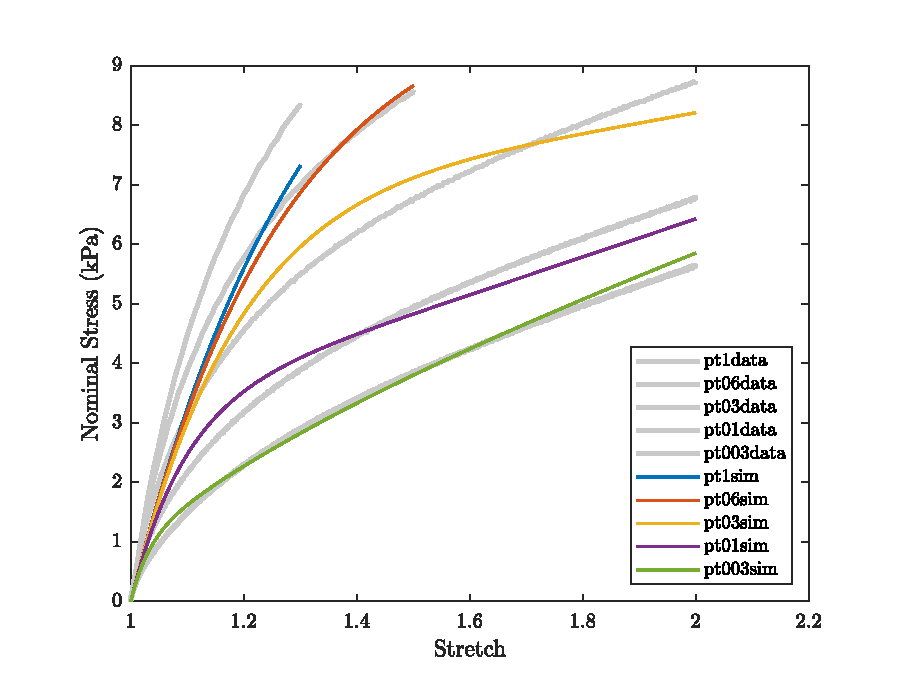
\includegraphics[width = 0.85\textwidth]{Optimization1EL_NR_all}} \label{fig:parameter_optimization_1EL_all}\\
    \caption[Parameter identification 1]{Parameter identification of viscoelastic material model with one relaxation mechanisms \((k=1)\) fit to (a) the experiment with stretch rate \(0.06s^{-1}\) and (b) all the five experiments together}
    \label{fig:parameter_optimization_1EL}
\end{figure}

Next, the viscoelastic material models with two \((k=2)\) or three \((k=3)\) relaxation mechanisms were considered. Even though, it was computationally more expensive to solve the optimization problem \cref{eq:constrained_optimization_cost}, it was possible to find a set of suitable parameters that would fit the material response to all the experiments together. As can be seen in \cref{fig:parameter_optimization} the response from the model with three relaxation mechanisms \((k=3)\) fits better to the experimental data. However, since certain material model parameters have no physical meaning when considered individually, the optimization problem provided different solutions when different starting points \((\bm{x}_{p})_{0}\) in the parameter space were considered. Moreover, as can be seen from  optimized parameter sets (a) and (b) in \cref{tab:opt_param_sets}, it was found that the bulk  \(\K{}, \km^{1}, \km^{2}\) for the elastic and inealstic parts in the model with two relaxation mechanisms (2EL) had little to no effect on the parameter optimization procedure. 


\begin{figure}[htpb]
    \centering
    \subfloat[]{\includegraphics[width = 0.85\textwidth]{Optimization2EL_all}} \label{fig:parameter_optimization_2EL} 
    \subfloat[]{\includegraphics[width = 0.85\textwidth]{Optimization3EL_all}} \label{fig:parameter_optimization_3EL}\\
    \caption[Parameter identification 2]{Parameter identification of viscoelastic material model (a) with two relaxation mechanisms \((k=2)\) and (b) with three relaxation mechanisms \((k=3)\) considering \(J=1\) and \(\lambda_{2,3} = \frac{1}{\sqrt{\lambda_1}}\)}
    \label{fig:parameter_optimization}
\end{figure}

\begin{figure}[htpb]
    \centering
    \subfloat[]{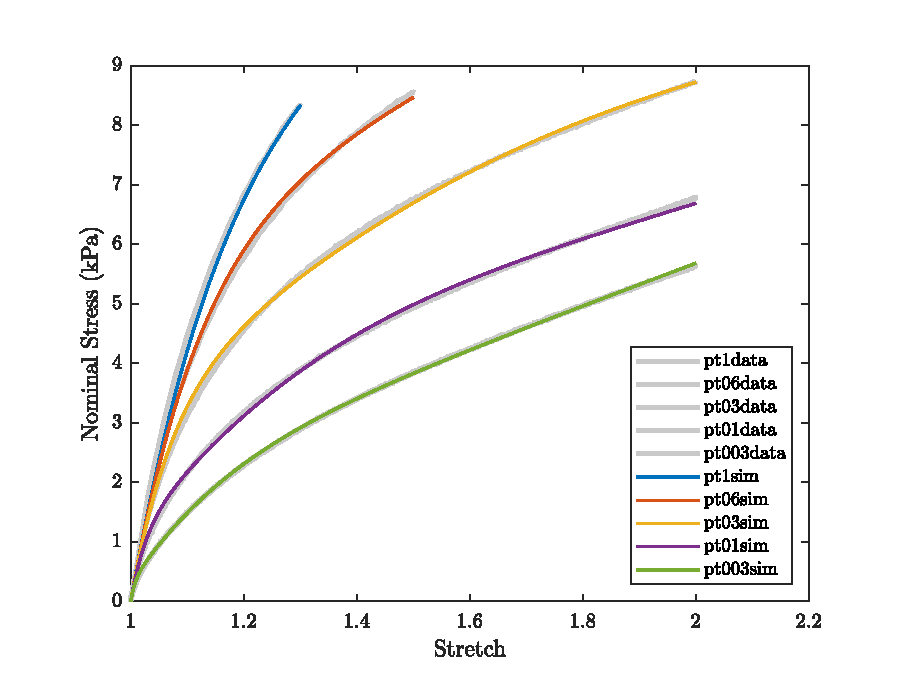
\includegraphics[width = 0.85\textwidth]{Optimization2EL_NR_all.eps}} \label{fig:parameter_optimization_nr_2EL} 
    \subfloat[]{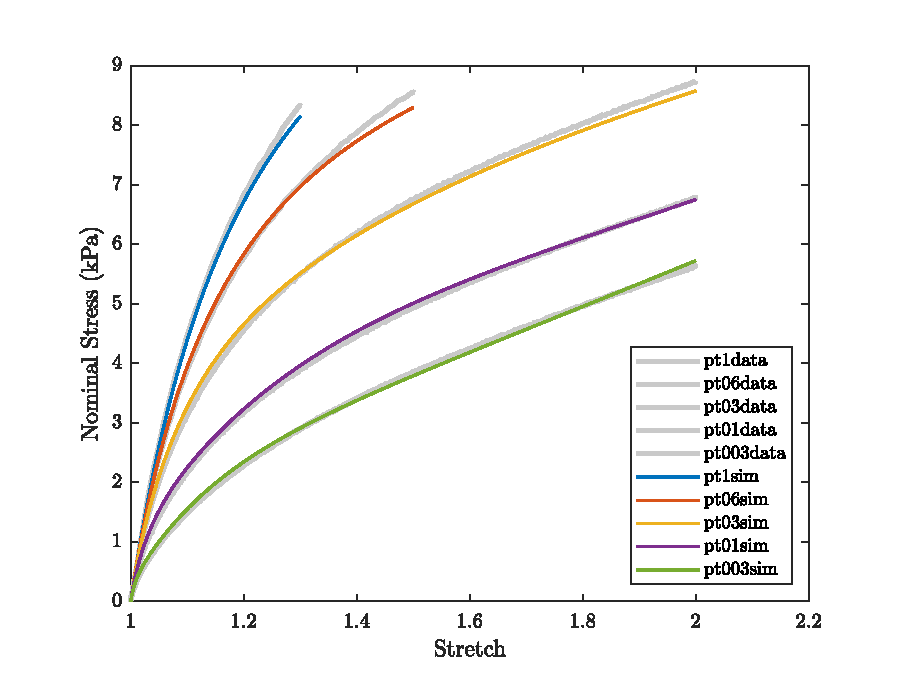
\includegraphics[width = 0.85\textwidth]{Optimization3EL_NR_all.eps}} \label{fig:parameter_optimization_nr_3EL}\\
    \caption[Parameter identification 3]{Parameter identification of viscoelastic material model (a) with two relaxation mechanisms \((k=2)\) and (b) with three relaxation mechanisms \((k=3)\) satisfying the condition \(\mathrm{P}_{22,33} = 0\)}
    \label{fig:parameter_optimization_nr}
\end{figure}


\begin{figure}[htbp]
    \centering
    \includegraphics[width=0.85\textwidth]{Optimization2EL_NRred_all.eps}
    \caption[Parameter identification 4]{Parameter identification for a viscoelastic material model with two relaxation mechanisms \((k=2)\) and a reduced parameter set}%
    \label{fig:parameter_optimization_red}
\end{figure}

Furthermore, the cost function was updated such that the stresses in the transverse direction would be zero in order to exactly mimic the uniaxial tension experiment. It must be noted that, the root-finding procedure (Newton-Raphson's method), that was necessary to achieve this condition, led to a tremendous increase in the number of computations performed within the cost function. Nevertheless, using this revised cost function, it was possible find a set of suitable parameters for the models with two \((k=2)\) and three \((k=3)\) relaxation mechanisms that simulated a response which was in close agreement to experimental data. Here, the response of the model with two relaxation mechanisms \((k=2)\) fit the experimental data better as can be seen in \cref{fig:parameter_optimization_nr}. For the model with one relaxation mechanism \((k=1)\), however, even after the cost function update, it was still not possible to find a set of parameters to fit the simulation response to all the experiments together. 

Finally, in an attempt to further reduce the number of model parameters, the viscous parameters \((\mum)^{k}, (\am{})^{k}, (\km{})^{k}\) were chosen to be equal to elastic parameters \(\mu, \alpha, \K\) respectively, as is sometimes done in literature \cite[][see Sec. 5]{Reese1998Sep}. For the model with two relaxation mechanisms\((k=2)\), using this methodology was found to be ineffective. Again as can be seen in \cref{fig:parameter_optimization_red}, the model rendered itself to be very simple to characterize the uniaxial tension experiments of the hydrogel. The sets of optimized parameters for all the optimization procedures carried out are summarized in \cref{tab:opt_param_sets}.

 


{\renewcommand{\arraystretch}{1.5}%
\begin{table}[htbp]
    \centering
    \begin{tabular}{cS[table-format=5.4]S[table-format=5.4]S[table-format=5.4]S[table-format=5.4]S[table-format=5.4]}
        \toprule
           &  {\text{2EL\({}_{1}\)}} &  {\text{2EL\({}_{2}\)}} &  {\text{2EL\({}_{\text{NR}}\)}} &  {\text{3EL}} &  {\text{3EL\({}_{\text{NR}}\)}} \\ \midrule   
        \(\bm{x}_{p}\)    &  {\text{(a)}} &  {\text{(b)}} &  {\text{(c)}} &  {\text{(d)}} &  {\text{(e)}} \\ \midrule   
        \(\mu\)           &  0.0040       &     0.0040    & 0.0026        &     0.0039    &     0.0024	  \\
        \(\alpha\)        &  2.1471       &     2.1474    & 2.1478        &     2.1578    &     2.2817	  \\ 
        \(\K\)            &  4.0000       &     40.0000   & 29.4615       &     40.0000   &     5.2712	  \\
        \(\mum^{1}\)      &  0.0686       &     0.0664    & 0.0643        &     0.0414    &     0.1182	  \\
        \(\am^{1}\)       &  0.5827       &     0.6011    & 0.4168        &     0.8837    &     0.1168	  \\
        \(\km^{1}\)       &  6.0000       &     60.0000   & 61.3862       &     59.9990   &     25.7008   \\
        \(\tau_{r}^{1}\)  &  3158.0       &     1.3159    & 1.2985        &     0.4912    &     0.3146	  \\
        \(\mum^{2}\)      &  0.0017       &     0.0017    & 0.0011        &     0.0042    &     0.1340	  \\
        \(\am^{2}\)       &  3.5330       &     3.5302    & 3.5251        &     3.5012    &     0.1376	  \\ 
        \(\km^{2}\)       &  5.0000       &     25.0000   & 29.0539       &     60.0006   &     14.4123   \\ 
        \(\tau_{r}^{2}\)  & 36.9815       &     36.9446   & 36.5179       &     3.3429    &     1.5602	  \\ 
        \(\mum^{3}\)      &     \text{-}  &     \text{-}  &    \text{-}   &     0.0014    &     0.0032	  \\
        \(\am^{3}\)       &     \text{-}  &     \text{-}  &    \text{-}   &     3.4523    &     1.7457	  \\ 
        \(\km^{3}\)       &     \text{-}  &     \text{-}  &    \text{-}   &     24.9999   &     2.7381	  \\ 
        \(\tau_{r}^{3}\)  &     \text{-}  &     \text{-}  &    \text{-}   &     45.9230   &     26.4516   \\ 
        \bottomrule
    \end{tabular}
    \caption[Optimized parameter sets]{Optimized parameter sets for the viscoealstic material model for the dual cross-link self-healing hydrogel.
    \newline \((k)\)EL stands for a model with \(k\) relaxation mechanisms \newline \((\bullet)_{\text{NR}}\) stands for models using cost function with the modified root-finding (Newton-Raphson's) procedure \cref{eq:optimization_NR}}
    \label{tab:opt_param_sets}
\end{table}}



